% XCircuit output "bloques.tex" for LaTeX input from bloques.eps
\def\putbox#1#2#3#4{\makebox[0in][l]{\makebox[#1][l]{}\raisebox{\baselineskip}[0in][0in]{\raisebox{#2}[0in][0in]{\scalebox{#3}{#4}}}}}
\def\rightbox#1{\makebox[0in][r]{#1}}
\def\centbox#1{\makebox[0in]{#1}}
\def\topbox#1{\raisebox{-0.60\baselineskip}[0in][0in]{#1}}
\def\midbox#1{\raisebox{-0.20\baselineskip}[0in][0in]{#1}}
   \scalebox{1}{
   \normalsize
   \parbox{8.94792in}{
   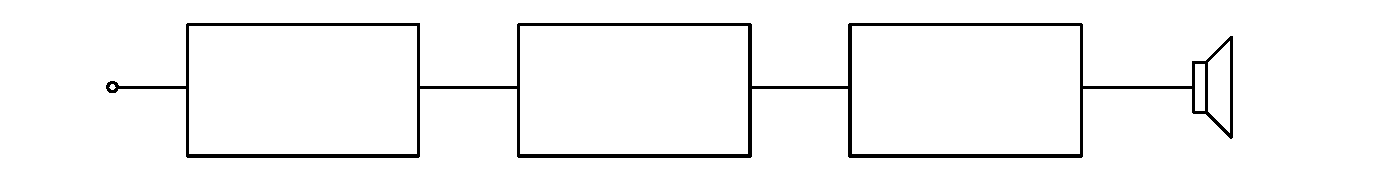
\includegraphics[scale=1]{bloques}\\
   % translate x=1016 y=-168 scale 0.38
   \putbox{1.31in}{0.68in}{1.20}{Comparador}%
   \putbox{1.31in}{0.43in}{1.20}{Baja ganancia}%
   \putbox{1.43in}{0.18in}{1.20}{de tension}%
   \putbox{3.47in}{0.68in}{1.20}{Amplificacion}%
   \putbox{3.60in}{0.47in}{1.20}{de tension }%
   \putbox{3.81in}{0.22in}{1.20}{VAS}%
   \putbox{5.85in}{0.68in}{1.20}{Ganancia}%
   \putbox{5.81in}{0.47in}{1.20}{de potenica}%
   \putbox{0.06in}{0.60in}{1.20}{Entrada}%
   \putbox{8.22in}{0.56in}{1.20}{Carga}%
   \putbox{8.22in}{0.35in}{1.20}{Parlante}%
   } % close 'parbox'
   } % close 'scalebox'
   \vspace{-\baselineskip} % this is not necessary, but looks better
